\documentclass[USenglish]{article}	
% for 2-column layout use \documentclass[USenglish,twocolumn]{article}

\usepackage[utf8]{inputenc}				%(only for the pdftex engine)
%\RequirePackage[no-math]{fontspec}[2017/03/31]%(only for the luatex or the xetex engine)
\usepackage[big,online]{dgruyter}	%values: small,big | online,print,work
\usepackage{lmodern} 
\usepackage{microtype}
\usepackage[numbers,square,sort&compress]{natbib}
\usepackage{algorithm}
\usepackage[utf8]{inputenc} % allow utf-8 input
%\usepackage[english]{babel}	% локализация и переносы
%\usepackage[T1]{fontenc}    % use 8-bit T1 fonts
\usepackage{booktabs}       % professional-quality tables
\usepackage{amsfonts}       % blackboard math symbols
\usepackage{nicefrac}       % compact symbols for 1/2, etc.
\usepackage{microtype}      % microtypography
\usepackage{lipsum}		% Can be removed after putting your text content
\usepackage{graphicx}
\usepackage{natbib}
\usepackage{doi}
\usepackage{amsmath}
\usepackage{amsthm}
\usepackage{amssymb}
\usepackage{mathtools}
\usepackage{algorithm}
\usepackage{algpseudocode}
\usepackage{appendix}


\graphicspath{{pictures/}, {images/}, {}}
\DeclareGraphicsExtensions{.pdf,.png,.jpg}

% Цвета 
\usepackage[dvipsnames]{xcolor}
\usepackage{color}   


% New theorem-like environments will be introduced by using the commands \theoremstyle and \newtheorem.
% Please note that the environments proof and definition are already defined within dgryuter.sty.
\theoremstyle{dgthm}
\newtheorem{theorem}{Theorem}
\newtheorem{assumption}{Assumption}
\newtheorem{corollary}{Corollary}
\newtheorem{proposition}{Proposition}
\newtheorem{lemma}{Lemma}
\newtheorem{assertion}{Assertion}
\newtheorem{result}{Result}
\newtheorem{conclusion}{Conclusion}

\theoremstyle{dgdef}
\newtheorem{definition}{Definition}
\newtheorem{example}{Example}
\newtheorem{remark}{Remark}



\begin{document}

	
%%%--------------------------------------------%%%
	\articletype{Research Article}
	\received{Month	DD, YYYY}
	\revised{Month	DD, YYYY}
  \accepted{Month	DD, YYYY}
  \journalname{De~Gruyter~Journal}
  \journalyear{YYYY}
  \journalvolume{XX}
  \journalissue{X}
  \startpage{1}
  \aop
  \DOI{10.1515/sample-YYYY-XXXX}
%%%--------------------------------------------%%%

\title{On methods with preconditioning and weight decaying}
\runningtitle{Preconditioning and weight decaying}
%\subtitle{Insert subtitle if needed}

\author[1]{Kreinin Matvei}
\author[1]{Babkin Petr}
\author[1]{Statkevich Ekaterina} 
\author[2]{Beznosikov Aleksandr}
\author[2]{Gasnikov Alexander}
\runningauthor{Babkin, Kreinin and Statkevich}

\affil[1]{\protect\raggedright 
Moscow Institute of Physics and Technology, Phystech School of Applied Mathematics and Computer Science, Moscow, Russia, e-mail: kreinin.mv@phystech.edu, babkin.pk@phystech.edu, statkevichk@bk.ru}

\affil[2]{\protect\raggedright 
Moscow Institute of Physics and Technology, Phystech School of Applied Mathematics and Computer Science, Moscow, Russia, e-mail:  beznosikov.an@phystech.edu, gasnikov@yandex.ru}
%\communicated{...}
%\dedication{...}
	
\abstract{This paper investigates the convergence behavior of optimization methods with preconditioning that utilize weight decay regularization, specifically focusing on popular variants such as AdamW and OASIS.
We explore different alternatives to these method, with the goal of investigating their convergence speed and accuracy.
Also we conduct experiments on benchmark datasets and models in order to compare them on practice.
Overall, our study provides insights into the design of regularization techniques methods with preconditioning.}

\keywords{Adam, AdamW, OASIS, Regularization, Weight Decay, Optimization}

\maketitle
	
	
\section{Introduction}
\label{sec:introduction}

A huge part of machine learning is based on the unconstrained optimization problem
\begin{equation}
    \label{eq:general}
	\min_{w \in \mathbb{R}^d} f(w).
\end{equation}
Problems of the form \eqref{eq:general} cover a plethora of applications, including empirical risk minimization \citep{chapelle2000vicinal},
deep learning \citep{lecun2015deep}, and supervised learning \citep{cunningham2008supervised} tasks such as regularized least squares \citep{rifkin2007notes} or logistic regression \citep{shalev2014understanding}.

The classic base method for solving the optimization problem \eqref{eq:general} is a gradient descent

\begin{equation}
    \label{GD}
	w_{t+1} = w_t - \eta \nabla f(w_t),
\end{equation}
But the minimization problem \eqref{eq:general} can be difficult to solve, particularly when the number of training samples or problem dimension is large.
In such cases, evaluating the full gradient on every iteration in the context of gradient descent becomes prohibitively expensive, especially considering that gradient descent often requires numerous iterations to converge.
In modern machine learning, especially with the advent of deep learning, there is a growing interest in tackling large and more complex problems.
For such cases stochastic gradient descent \citep{robbins1951stochastic} became popular solution.
% Despite its simplicity, it proved itself to be an efficient and effective optimization method.

Over time, optimization methods have continuously advanced and evolved, becoming more sophisticated and intricate.
One prominent aspect of optimization is the efficient selection of the step size during the iterative process.
Adaptive methods with gradient scaling dynamically adjust the step size based on the gradient information. This adaptive behavior, applied to each variable, improves the optimization process by efficiently navigating complex landscapes and ensuring optimal progress for each variable \citep{hazan2007adaptive}.
In particular, these methods have gained significant popularity in the field of machine learning, where high-dimensional problems are prevalent \citep{zhang2018three, yao2021adahessian}.

In more details, methods with scaled gradient refer to techniques that involve preconditioning the gradient of a problem by a specific matrix $D_t$, which enables the gradient to take into account the geometry of the problem. Generally, the step of preconditioned algorithms can be expressed as a following modernization of step \eqref{GD}:
\begin{equation}
    w_{t+1} = w_t - \eta \cdot D_t^{-1} g_t,
\end{equation}
where $g_t$ is an unbiased stochastic gradient.
The idea of using the scaling matrix refers to Newton's method, where $D_t = \nabla^2 f(w)$. However calculating and reversing hessian poses significant challenges, thus necessitating the utilization of certain heuristics as replacements. Such techniques are exemplified in Adagrad \citep{duchi2011adaptive}, Adam \citep{kingma2014adam}, RMSProp, OASIS \citep{goldberg2011oasis} and so forth, where the computation strategies for $D_t$ do not necessitate the evaluation of hessian. For example, Adagrad presents preconditioning in the form:
$$ D_t = \text{diag} \left\{ \sqrt{\sum_{t'=0}^t{g_{t'} \odot g_{t'}}} \right\}, $$
where $\odot$ is a Hadamard product. In fact this approach uses only stochastic gradients.
RMSProp and Adam utilize a similar idea:
$$ D_t^2 = \beta D_{t-1}^2 + (1 - \beta) \text{diag} \left\{ g_{t} \odot g_{t} \right\} $$
where $\beta$ represents the degree of consideration given to previous iterations \citep{kingma2014adam}.
OASIS uses another approach:
$$ D_t = \text{diag} \left\{ z_k \odot \nabla^2 f(w_t) z_k \right\}, $$
where here $z_k$ is a random vector of Randamaher distribution, i.e. each element of the vector $z_k^i \in \{-1, 1\}$ with probabilities $\frac{1}{2}$ \citep{goldberg2011oasis}. Hear the hessian matrix appears to be employed, but it is actually approximated through scalar function differentiation.

Despite the advantages of preconditioning methods, they are prone to overfitting, thus necessitating their combined application with regularization. This approach has been widely applied to various machine learning problems, including image classification \citep{zhu2017learning}, speech recognition \citep{zhou2017improved}, and natural language processing \citep{wu2022stgn}, and has shown its effectiveness in improving the generalization capability of neural networks \citep{girosi1995regularization}. With regularization, problem \eqref{eq:general} is reformulated as
\begin{equation} \label{F_big}
	\min_{w \in \mathbb{R}^d} F(w) := f(w) + r(w),
\end{equation}
where $r$ is a regularizer function.

In methods with preconditioning appears to be several ways to include regularization.
We can include regularizer $r$ in $g_t$ calculation thus it will be taken into consideration while calculating $D_t$. This method is equal to considering optimization problem \eqref{F_big}.
Or we can include regularizer only on last step, decreasing norm of $w$ \citep{loshchilov2017decoupled}.
This way of regularization is called weight decay and surprisingly turns out to be more efficient in practical problems.
There is another ways of considering regularizer which will be discussed further in the paper.

Despite their practical efficiency, methods incorporating weight decay show relatively limited theoretical analysis.
As a result, a number of research inquiries arise:
\begin{itemize}
    \item \textit{Do methods utilizing weight decay and a preconditioning technique converge?}
    \item \textit{If so, what is the rate of convergence?}
    \item \textit{To what solution do they converge?}
\end{itemize}


\subsection{Related works}
%The most common regularization technique is $\ell_2$-regularization, defined as $r(w_t) = \frac{\lambda}{2} ||w_t||^2$, which yields $\nabla r (w_t) = \lambda \cdot w_t$.
%In this case, the weight decay regularization achieves its name.
%It only serves to reduce the norm of the weight vector, through the subtraction of $\eta \cdot w_t$ in the final step.

Stochastic methods have an extensive theory of convergence \citep{schneider2007stochastic, heyman2004stochastic, spall1998implementation}, whereas methods involving preconditioning are relatively new and have a limited history of investigations.
In one of the pioneering papers on preconditioning \citep{duchi2011adaptive}, the authors conducted a meticulous analysis of Adagrad's convergence theory.
However, in more recent papers such as those discussing RMSProp \citep{rmsprop} or Adam \citep{kingma2014adam}, little attention was given to theoretical aspects or the existing theory may contain inaccuracies.
Over time, mistakes were rectified, leading to the development of comparatively robust convergence theories for preconditioning methods \citep{reddi2019convergence, defossez2020simple}.
In another study, Loshchilov and Hutter \citep{loshchilov2017decoupled} investigated the properties of the Adam and AdamW algorithms in terms of hyperparameters and also explored restart techniques.
Zhang et al. \citep{zhang2019lookahead} delved into the lookahead mechanism of Adam.
More recently, convergence theories have been established for modern methods such as OASIS \citep{goldberg2011oasis, sadiev2022stochastic}.
Additionally, a theory addressing time-varying preconditioning has also emerged \citep{beznosikov2022scaled}.
Nevertheless, numerous questions in this field remain unanswered.
A few of these inquiries are formulated at the end of the preceding paragraph and examined in our paper.

\if0
\begin{equation}
w_{t+1} = w_t - \eta \cdot D_t^{-1} \nabla f(w_t) - \eta \cdot \nabla r(w_t),
\end{equation}
\fi

\subsection{Contributions}

In general, our paper provides insight into comparison of different consideration ways of regularization is methods with preconditioning. Here, we provide a brief summary of our main contributions:

\begin{itemize}
    \item \textbf{Novel approach to regularization in preconditioning.} We propose a novel method of integrating regularization into preconditioning algorithms, where we utilize identical step sizes for the objective function and the regularizer. At the same time regularizer does not impact the computation of $D_t$.
    
    \item \textbf{Proof of preconditioned methods with weight decay convergence.}  In this discourse, we elucidate the convergence properties of preconditioned optimization algorithm with regularization, particularly when supplemented with weight decay mechanisms. Our non-convex theoretical exposition revolves around the foundational assumptions encompassing the smoothness of the function \eqref{ass:smoothness}. We achieve different convergence speed assessments based on the PL-condition \eqref{ass:plcondition} and conducte a stochastic analysis based on assumption \eqref{ass:expectations}. Through meticulous analysis, we aim to furnish robust guarantees affirming the convergent behavior of such preconditioned methods under the specified conditions.

    \item \textbf{Investigation of loss function behavior.} We conducted a comparative study on the convergence rate of the Adam and Adam with weight decay (AdamW). We observed that AdamW converges towards a distinct target function. Subsequently, we conducted an analysis of these target function.
    
    %\item \textbf{Competitive numerical results.} We investigate the empirical performance of Adam's variation including new one on a variety of standard machine learning tasks, including logistic regression.
\end{itemize}

\section{Main part}

\subsection{Notation:}
\begin{itemize}
    \item $L_f$ -- lipschitz constant of function $f$, $\forall x, y \in \mathbb{R}^d \rightarrow $ 	$f(x) \leq f(y) + \langle \nabla f(y), x-y \rangle + \frac{L_f}{2} \|x - y\|^2$
    \item $|| x || = \langle x, x \rangle$  - the second norm, where $x \in \mathbb{R}^d$
    \item $|| x ||_A^2 = x^TAx$, where $x \in \mathbb{R}^d, A \in \mathbb{R}^{d \times d}$
    \item A -- matrix $\in \mathbb{R}^{d \times d}$, $A^{-1}$ -- inverse matrix to A $\in R^{d \times d}$.
    \item $\textrm{diag} \left\{ \beta_1 \ldots, \beta_d \right\}$ -- diagonal matrix with elements $\beta_1, ..., \beta_d$
    
\end{itemize}


\subsection{Weight decay and how to use it with preconditioning}
As it was mentioned above, in preconditioned methods, there exist several techniques for incorporating regularization into the optimization process.
In this study, we consider three different approaches, which are illustrated in \hyperref[alg:precond]{Algorithm 1} using different colors.

\begin{algorithm}[H]
    \caption{Different ways of using preconditioning for regularized problem}
    \label{alg:precond}
    
    \begin{algorithmic}
            \Require{$\eta$ $-$ learning rate, $f$ $-$ objective function}
            
            \While {$w$ not converged}
            \State $t = t+1$
            \State $g_t \gets$ stochastic gradient of $f$
            \State $\textcolor{blue}{g_t \gets g_t + \nabla r(w_t)}$ \hfill \textcolor{blue}{standart regularization}
            \State $D_t \gets$ preconditioning matrix, based on $g_t$

            \State \textcolor{blue}{$w_t \gets w_{t-1} - \eta \cdot D_t^{-1}g_t $} \hfill \textcolor{blue}{standart regularization}, 
            \State \textcolor{orange}{$w_t \gets w_{t-1} - \eta \cdot D_t^{-1} \left(g_t +\nabla r(w_t) \right)$} \hfill \textcolor{orange}{scaled weight decay}, 
            \State \textcolor{red}{$w_t \gets w_{t-1} - \eta \cdot D_t^{-1} g_t  - \eta \cdot \nabla r(w_t)$} \hfill \textcolor{red}{weight decay}, 
            \EndWhile
    \end{algorithmic}
\end{algorithm}

To be more specific, the first regularization technique illustrated in \textcolor{blue}{blue} involves simply adding the regularization term to the objective function. This regularizer is included in the pseudo-gradient and factored into the calculation of $D_t$. In essence, this approach involves applying the basic preconditioning method to the problem \eqref{F_big}.
The second regularization technique, shown in \textcolor{orange}{orange}, is a novel approach. Although regularizer term does not affect its computation of preconditioner $D_t$, it is added before applying $D_t$. That means that learning rate is adopted in the same way for gradient and regularizer.
The last regularization approach we consider is known as weight decay, illustrated by the color \textcolor{red}{red} in Algorithm \ref{alg:precond}.
Similar to the second method, matrix $D_t$ is calculated without using regularizer and this method incorporates the regularizer during the algorithmic step, avoiding interference of regularization with the preconditioning stage.

Overall, it is important to carefully consider the impact of regularization when designing optimization algorithms, and we hope that our investigation of this techniques will prove useful to researchers in the field.


\subsection{Convergence speed of preconditioning methods with weight decay}

We set ourselves a goal to estimate a convergence speed of methods with preconditioning with weight decay regularization.
Although step of methods with weight decay seems simple, it can be viewed in a rather unexpected way. We can put $D_t^{-1}$ out of brackets which gives
\begin{equation}
w_{t+1} = w_t - \eta \cdot D_t^{-1} (\nabla f(w_t) + D_t \nabla r(w_t)).
\end{equation}
That suggests the need to introduce a function $\tilde{r}$ such that $\nabla \tilde{r}(w) = D_t \nabla r(w)$ and new target function
\begin{equation} \label{F_tilde}
    \tilde{F}(w) := f(w) + \tilde{r}(w),
\end{equation}
where new target function $\widetilde{F}$ changes at every time-step, because $D_t$ changes at every time-step.

New adaptive regularizer $\widetilde{r}$ does not exist in the general case. Therefor we impose restrictions on initial regularizer and preconditioner structure. That is framed in the following assumptions.

\begin{assumption}{(Regularizer structure)}
    \label{ass:regstruct}
    Regularizer $r$ is separable, i.e. it can be viewed in the following form:
    $$r(w) = \sum_{i=1}^d r_i(w_i).$$
\end{assumption}

\begin{assumption}{(Preconditioner structure)}
    \label{ass:precondstruct}
    Preconditioner $D_t$ can be viewed in the following form:
\end{assumption}
$$ D_t = \textrm{diag} \left\{ d_t^1 \ldots, d
_t^d \right\}.$$

Although these assumptions are strict, they hold for every mentioned method with preconditioning and applicable regularizers.

The convergence speed is typically measured in terms of the number of iterations required to reach a certain level of error.
To obtain estimates on the number of iterations required to converge to a given error, we must impose certain assumptions on the function.
Throughout theoretical analysis we assume that $f : \mathbb{R}^d \rightarrow \mathbb{R}$ is $L-$smooth and twice differentiable.
Additionally we imply a PL-condition to make another evaluation concerning speed of convergence.

\begin{assumption}{($L$-smoothness)} 
\label{ass:smoothness}
\begin{itemize}
    \item 	The gradients of $f$ are $L_f$-Lipschitz continuous $\forall w \in \mathbb{R}^d$, i.e. there exists a constant $L_f > 0$ such that $\forall x, y \in \mathbb{R}^d$,
    	\begin{equation*}
    		f(x) \leq f(y) + \langle \nabla f(y), x-y \rangle + \frac{L_f}{2} \|x - y\|^2.
    	\end{equation*}
    \item    The gradient of $r$ is $L_r$-Lipschitz continuous $\forall w \in \mathbb{R}^d$, i.e. there exists a constant $L_r > 0$ such that $\forall x, y \in \mathbb{R}^d$,
	\begin{equation*}
		r(x) \leq r(y) + \langle \nabla r(y), x-y \rangle + \frac{L_r}{2} ||x - y||^2.
	\end{equation*}
\end{itemize}
\end{assumption}

\begin{assumption}{(PL--condition)}
\label{ass:plcondition}
	There exists $\mu > 0$, such that $\forall w \in \mathbb{R}^d$
    $$||\nabla f(w) || \geq 2 \mu (f(w) - f^*).$$
\end{assumption}

We use popular restriction on the preconditioner, which is framed in Assumption \ref{ass:preconditioned}.

\begin{assumption}{(Preconditioner)}
\label{ass:preconditioned}
Restrictions on preconditioner $D_t$
\begin{equation}
\alpha I \preccurlyeq D_t \preccurlyeq \Gamma I \Leftrightarrow \frac{I}{\alpha} \preccurlyeq D_t^{-1} \preccurlyeq \frac{I}{\Gamma}.
\end{equation}
\end{assumption}

It has been proven that this assumption holds for all modern algorithms with preconditioning like Adam, Adagrad, OASIS \citep{beznosikov2022scaled}.

In order to conduct a stochastic analysis we must include restrictions on the stochastic gradient of the function.
This is formalized in the following assumption \ref{ass:expectations}.

\begin{assumption}{(Expectations)}
\label{ass:expectations}
Restrictions on $D_t$ and $g_t$ are unbiased, i.e.
\begin{equation}
\mathbb{E} \left[ D_t \right] = D_t \text{ and }\mathbb{E}\left[ g_t \right] = \nabla f (w_t), \mathbb{E}\left[ ||g_t - \nabla f||^2 \right] \leq \sigma^2.
\end{equation}
\end{assumption}

With the assumptions \ref{ass:regstruct} and \ref{ass:precondstruct} we are able to prove existence of $\widetilde{r}$ and, consequently, $\widetilde{F}$. We frame that in the Lemma \ref{lemma:existence}. We only show existence, but not uniqueness of the function, but in our evaluations, $\widetilde{F}$ can be found up to a constant.

\begin{lemma}
\label{lemma:existence}
{(Existence of $\widetilde{r}$)}
    Suppose the Assumptions \ref{ass:regstruct}, \ref{ass:precondstruct} hold, the function $\widetilde{r}$ exists and has following form:
    $$\widetilde{r}(w) = \sum_{i=1}^d d_t^i r_i(w_i)$$
\end{lemma}

Using introduced Assumption \ref{ass:smoothness} we can guarantee smoothness for $\widetilde{r}$ and estimate its Lipschitz constant, which is formally framed and proved in Lemmas \ref{lemma:tildesmoothness}.

\begin{lemma}\label{lemma:tildesmoothness}{(L-smoothness of $\widetilde{r}$)}
Suppose the Assumptions \ref{ass:regstruct}, \ref{ass:precondstruct}, \ref{ass:smoothness} hold,
The gradient of $\widetilde{r}$ is $L_{\tilde{r}}$-continuous, i.e.  there exists a constant $L_{\tilde{r}} > 0$ such that $\forall x, y \in \mathbb{R}^d$,
    	\begin{equation*}
    		\widetilde{r}(x) \leq \widetilde{r}(y) + \langle \nabla \widetilde{r}(y), x-y \rangle + \frac{L_{\tilde{r}}}{2} ||x - y||^2,
    	\end{equation*}
     where $L_{\tilde{r}} = ||D_t|| L_r$
\end{lemma}

Using introduced assumptions we proved convergence of methods with preconditioning with weight decay regularization in general form. Our results are framed in Theorem \ref{theor:1} and Theorem \ref{theor:2}. Proofs of the theorems can be found in Appendix \ref{sec:appendix}.

\begin{theorem} 
    \label{theor:1}
    Suppose the Assumptions \ref{ass:smoothness}, \ref{ass:preconditioned} hold, let $\varepsilon > 0$ and let the step-size satisfy, where $L_f, L_{\tilde{r}}$ - lipschitz constants of functions $f$ and $\tilde{r}$, $\alpha I \preccurlyeq D_t \preccurlyeq \Gamma$
    \begin{equation*}
        \eta < \frac{2 \alpha}{L_f + \Gamma L_{\tilde{r}} \alpha}.
    \end{equation*}
    Then, the number of iterations performed by algorithms with preconditioning and weight decaying, starting from an initial point $w_0 \in \mathbb{R}^d$ with $\Delta_0 = \tilde{F}(w_0) - \tilde{F}^*$, required to obtain and $\varepsilon$-approximate solution of the convex problem \eqref{eq:general} can be bounded by
    \begin{equation*}
          T = \mathcal{O}\left( \frac{2\Delta_0 \Gamma \alpha } {\left(2\alpha - \left( L_f + \Gamma L_{\tilde{r}} \alpha \right)\eta \right) \eta \varepsilon} \right).
    \end{equation*}
\end{theorem}

\begin{theorem}
\label{theor:2}
    Suppose the Assumptions \ref{ass:smoothness}, \ref{ass:plcondition}, \ref{ass:preconditioned} hold, let $\varepsilon > 0$ and let the step-size satisfy, where $\alpha I \preccurlyeq D_t \preccurlyeq \Gamma$, $L_{\tilde{F}} = L_{f} + \Gamma L_{r}$, and $L_{F}, L_{r}$ - lipschitz constant of functions $f$ and $r$, 
    \begin{equation*}
        \eta \leq \frac{2 \alpha}{L_{\widetilde{F}}}.
    \end{equation*}
    Let $\tilde{F}^*$ be a solution of the optimization function. Then, the number of iterations performed by algorithms with preconditioning and weight decaying, starting from an initial point $w_0 \in \mathbb{R}^d$ with $\Delta_0 = \tilde{F}(w_0) - \tilde{F}^*$, required to obtain and $\varepsilon$-approximate solution of the convex problem \eqref{eq:general} can be bounded by
    \begin{equation*}
        T =  \mathcal{O}\left( \frac{\ln \frac{\Delta_0}{\epsilon}}{2 \mu \eta^2 \left(\frac{1}{\eta} - \frac{L_{\tilde{F}}}{2 \alpha} \right)} \right).
    \end{equation*}
\end{theorem}

\begin{theorem}
    Suppose the Assumptions \ref{ass:smoothness}, \ref{ass:plcondition}, \ref{ass:preconditioned}, \ref{ass:expectations} hold, let $\varepsilon > 0$ and let the step-size satisfy
    \begin{equation*}
        \eta \approx \sqrt{\frac{\left( \tilde{F}(w_0) - \tilde{F}(w_*) \right)\alpha}{L \sigma^2}}.
    \end{equation*}
    Let $\tilde{F}^*$ be a solution of the optimization function. Then, the number of iterations performed by algorithms with preconditioning and weight decaying, starting from an initial point $w_0 \in \mathbb{R}^d$ with $\Delta_0 = \tilde{F}(w_0) - \tilde{F}^*$, required to obtain and $\varepsilon$-approximate solution of the convex problem \eqref{eq:general} can be bounded by, where $L_{\tilde{r}}, L_{f}$ - lipschitz constant of functions $\tilde{r}$ and $f$, and $L_{\tilde{F}} = L_{f} + \Gamma L_{r}$
    
    \begin{equation*}
        T =  \mathcal{O}\left( \frac{\Gamma \Delta_0}{\left(\frac{1}{\eta} - \frac{ \Gamma L_{\tilde{r}}}{2} - \frac{\Gamma L_{\tilde{F} }L_{f}\eta^2}{2\alpha^2} \right) \varepsilon} \right).
\end{equation*}
    \label{theor:3}
\end{theorem}

These theorems establish the convergence of methods with preconditioning and weight decay under different assumptions, and further delineate their iterative rates. For our objectives, the simple act of convergence by these methods holds profound importance. 
However, characteristics of the solution $\widetilde{w}^*$  of a problem
\begin{equation} \label{F_tilde}
	\min_{w \in \mathbb{R}^d} \tilde{F}(w) = f(w) + \tilde{r}(w),
\end{equation}
to which this method converge demand a deeper exploration, which will be elucidated in the subsequent section.

\subsection{Solution of preconditioning methods with weight decay} 

 In the previous subsection we have proved convergence of preconditioned methods, however we have pointed out above that methods with weight decay does not converge to the initial optimization problem \eqref{F_big} solution $w^*$, but rather to a new solution $\widetilde{w}^*$ of a problem \eqref{F_tilde}. This observation is evidenced by the experiments detailed in Section \ref{subsec:experiments}.

Let us estimate the difference between solutions of problems \eqref{F_big} and \eqref{F_tilde}. This restriction is based on Assumptions \eqref{ass:smoothness} and properties of matrix $D_t$.

\begin{lemma}\label{lemma:lowerbondF}{(Lower bound)}
Suppose the Assumptions \ref{ass:regstruct}, \ref{ass:precondstruct} and \ref{ass:smoothness} holds, then difference between a solution $w^*$ of a problem \eqref{F_big} and a solution $\widetilde{w}^*$ of a problem \eqref{F_tilde} can be bounded below.
    \begin{equation*}
        \|\widetilde{w}^* - w^* \| L_F \geq \| \nabla r (\widetilde{w}^*) (I - D_t)\|
    \end{equation*}
\end{lemma}

Consequently, it can be observed that employing techniques such as preconditioning and weight decay yields convergence towards an alternate solution.
The discrepancy between these solutions is contingent upon the norm of the difference between $D_t$ and the identity matrix ($||D_t - I||$).
As a result, an analysis of the distribution of the elements of $D := \lim_{t \to \infty} D_t$ can provide insights into the convergence behavior of the weight decay method.


\section{Experiments}
\label{subsec:experiments}

We will consider two algorithms OASIS \citep{goldberg2011oasis} and Adam \citep{kingma2014adam}, and its variations. Their main difference is in the calculation of the pseudo hessian.
In Adam, the Hessian is a diagonal matrix consisting of squares of derivatives, in OASIS we have a stochastic Hessian, which is calculated through a random variable from the Randemacher distribution. 
We framed three methods of regularization for Adam and OASIS in Algorithm \ref{alg:genAdam} and Algorithm \ref{alg:OASIS} respectively.

\begin{algorithm}[H]
            \caption{Different ways of using Adam for regularized problem}
            \label{alg:genAdam}    
            \begin{algorithmic}
            \small{
            \Require{$\eta, \beta_1, \beta_2, \epsilon, f, r$}
            %\State $m_0 = 0$ -- 1-st moment vector
            %\State$v_0 = 0$ -- 2-nd moment vector
            \While {$\theta$ not converged}
            \State $t = t+1$
            \State $g_t = \nabla f(w_{t-1}) + $ \textcolor{blue}{$\nabla r(w_{t-1})$}\hfill \textcolor{blue}{AdamL2}
            \State $m_t = \beta_1 \cdot m_{t-1} + (1 - \beta_1) \cdot g_t$
            \State $v_t = \beta_2 \cdot v_{t-1} + (1 - \beta_2) \cdot g_t^2$
            \State $\hat{m_t} = \frac{m_t}{1-\beta_1^t} +$ \textcolor{orange}{$\nabla r(w_{t-1})$} \hfill \textcolor{orange}{AdamWH}
            \State $\hat{v_t} = \frac{v_t}{1-\beta_2^t}$ 
            \State $w_t = w_{t-1} - \eta \cdot \frac{\hat{m_t}}{\sqrt{v_t} + \epsilon} - $ \textcolor{red}{$\eta \nabla r(w_{t-1})$ } \hfill \textcolor{red}{AdamW}
            \EndWhile
            }
\end{algorithmic}
\end{algorithm}

\begin{algorithm}[H]
\caption{Different ways of using OASIS for regularized problem}\label{alg:OASIS}
\begin{algorithmic}
    \Require{$w_0, \eta_0, D_0, \theta_0 = + \infty$}    
    \State $w_1 = w_0 - \eta \hat{D_0}^{-1} \nabla f(w_0)$

    \For{$k = 1, 2, ...$}
    \State $g_k = \nabla f(w_k) +$ \textcolor{blue}{$\nabla r(w_{t-1})$}\hfill \textcolor{blue}{OASISL2} 
    \State $D_k = \beta D_{k-1} + (1-\beta_2) \cdot diag\left( z_k \odot \nabla^2 \left(f(w_k) + \textcolor{orange}{r(w_k)} \right) z_k \right)$ \hfill \textcolor{orange}{OASISWH}
    \State $(\hat{D_k})_{ii} = max \{|D_k|_{i, i} ; \alpha \}$, $\forall i = \overline{1, d}$
    \State $\eta_k = min \{ \sqrt{1 + \theta_{k-1}} \cdot \eta_{k-1}; \frac{||w_k - w_{k-1}||_{\hat{D_k}}}{2 ||\nabla f(w_k) - \nabla f(w_{k-1}) ||_{\hat{D_k}}^* } \}$
    \State $w_{k+1} = w_k - \eta_k g_k D_k^{-1}- $ \textcolor{red}{$\eta \nabla r(w_{t-1})$ } \hfill \textcolor{red}{OASISW} 
    \State $\theta_k = \frac{\eta_k}{\eta_{k-1}}$
    \EndFor
    
\end{algorithmic}
\end{algorithm}

The results of our computational experiments are presented in Figures \ref{fig:adams_errors} and \ref{fig:adams_special_errors}.
It can be observed that AdamW does not converge according to the basic criterion $||\nabla F(w_t)|| = \nabla f(w_t) + D_t \nabla r(w_t)||$, but it converges only by the special criterion $||\nabla \widetilde{F}(w_t) = ||\nabla f(w_t) + D_t \nabla r(w_t)||$.
Furthermore, it is noted that AdamW exhibits better convergence according to its own criterion.

\begin{figure}[H]
\begin{minipage}[h]{0.5\linewidth}
\centering
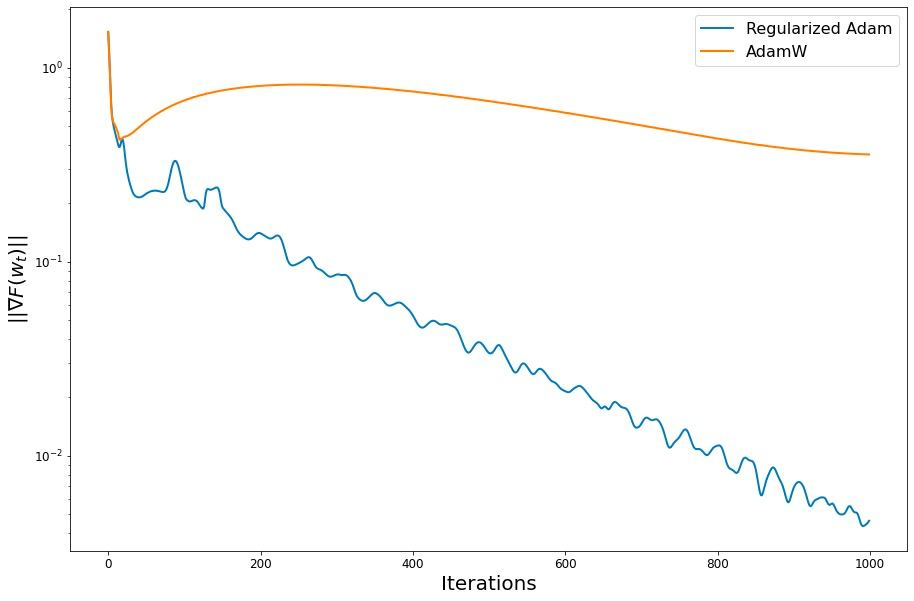
\includegraphics[width=\linewidth]{pictures/adams_errors.jpeg}
\captionsetup{justification=centering,margin=0.5cm}
\caption{Adam and AdamW with basic criterion}
\label{fig:adams_errors}
\end{minipage}
\hfill
\begin{minipage}[h]{0.5\linewidth}
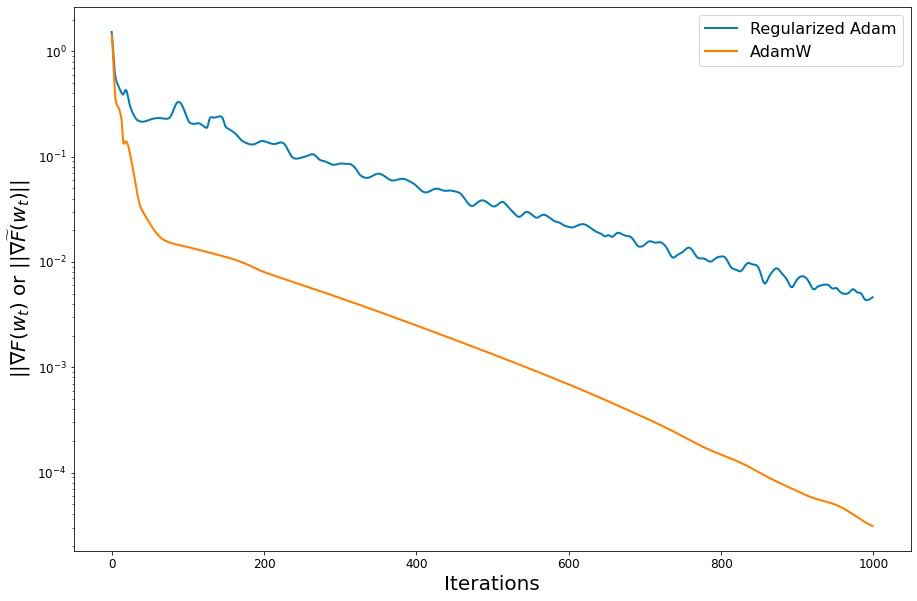
\includegraphics[width=\linewidth]{pictures/adams_special_errors.jpeg}
\captionsetup{justification=centering,margin=0.5cm}
\caption{Adam and AdamW with modified criterion}
\label{fig:adams_special_errors}
\end{minipage}
\end{figure}

We think that this observation can be an explanation for the fact that AdamW performs better in the applied problems.
The results of our experiments are presented below.
We trained the \href{https://pytorch.org/vision/main/models/generated/torchvision.models.resnet18.html}{ResNet18} \citep{he2015deep} on four different optimizators using \href{https://pytorch.org/docs/stable/generated/torch.optim.lr_scheduler.CosineAnnealingLR.html}{CosineAnnealingLr} on dataset \href{https://www.cs.toronto.edu/~kriz/cifar.html}{CIFAR10} \citep{li2017cifar10}.

\begin{figure}[H]
    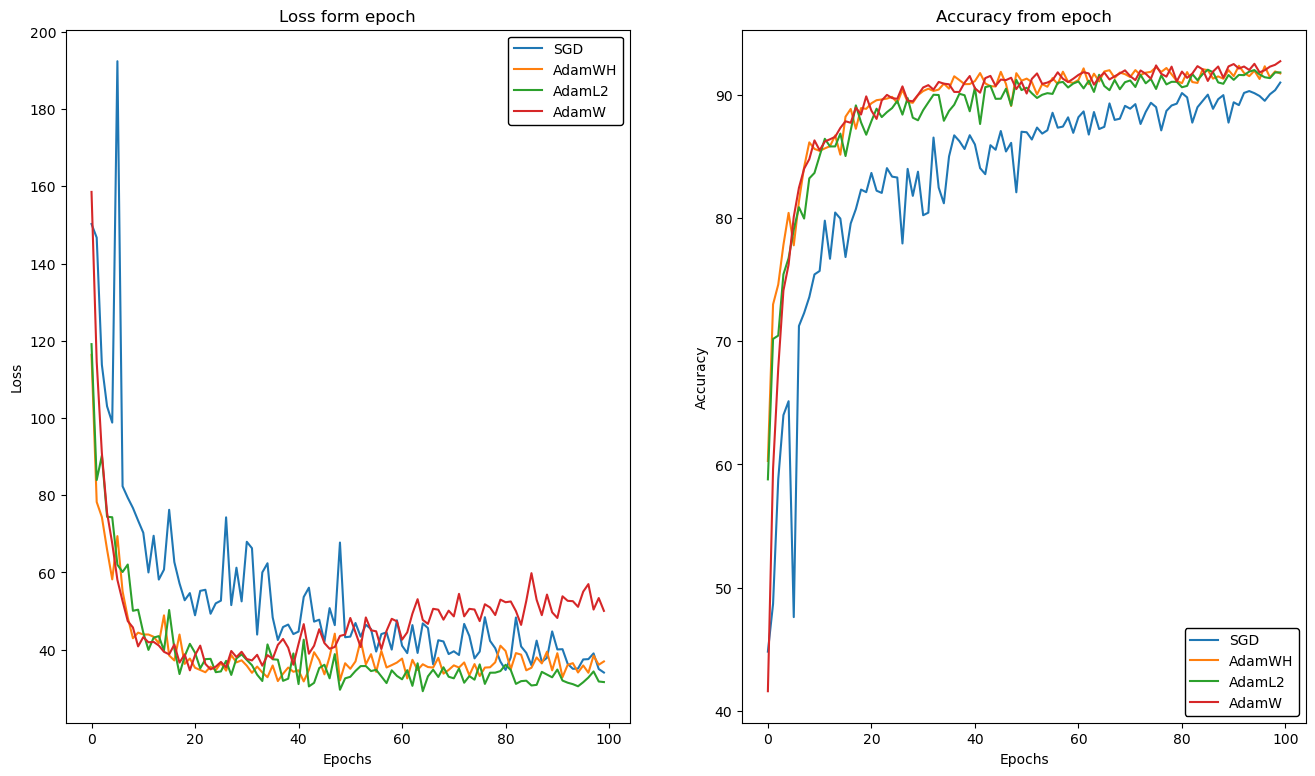
\includegraphics[width=\textwidth]{pictures/nn_results.png}
    \captionsetup{justification=centering,margin=2cm}
    \caption{Compare different optimization algorithms on dataset: CIFAR10}
        \label{fig:main_resnet18}
\end{figure}

\begin{figure}[H]
\centering
    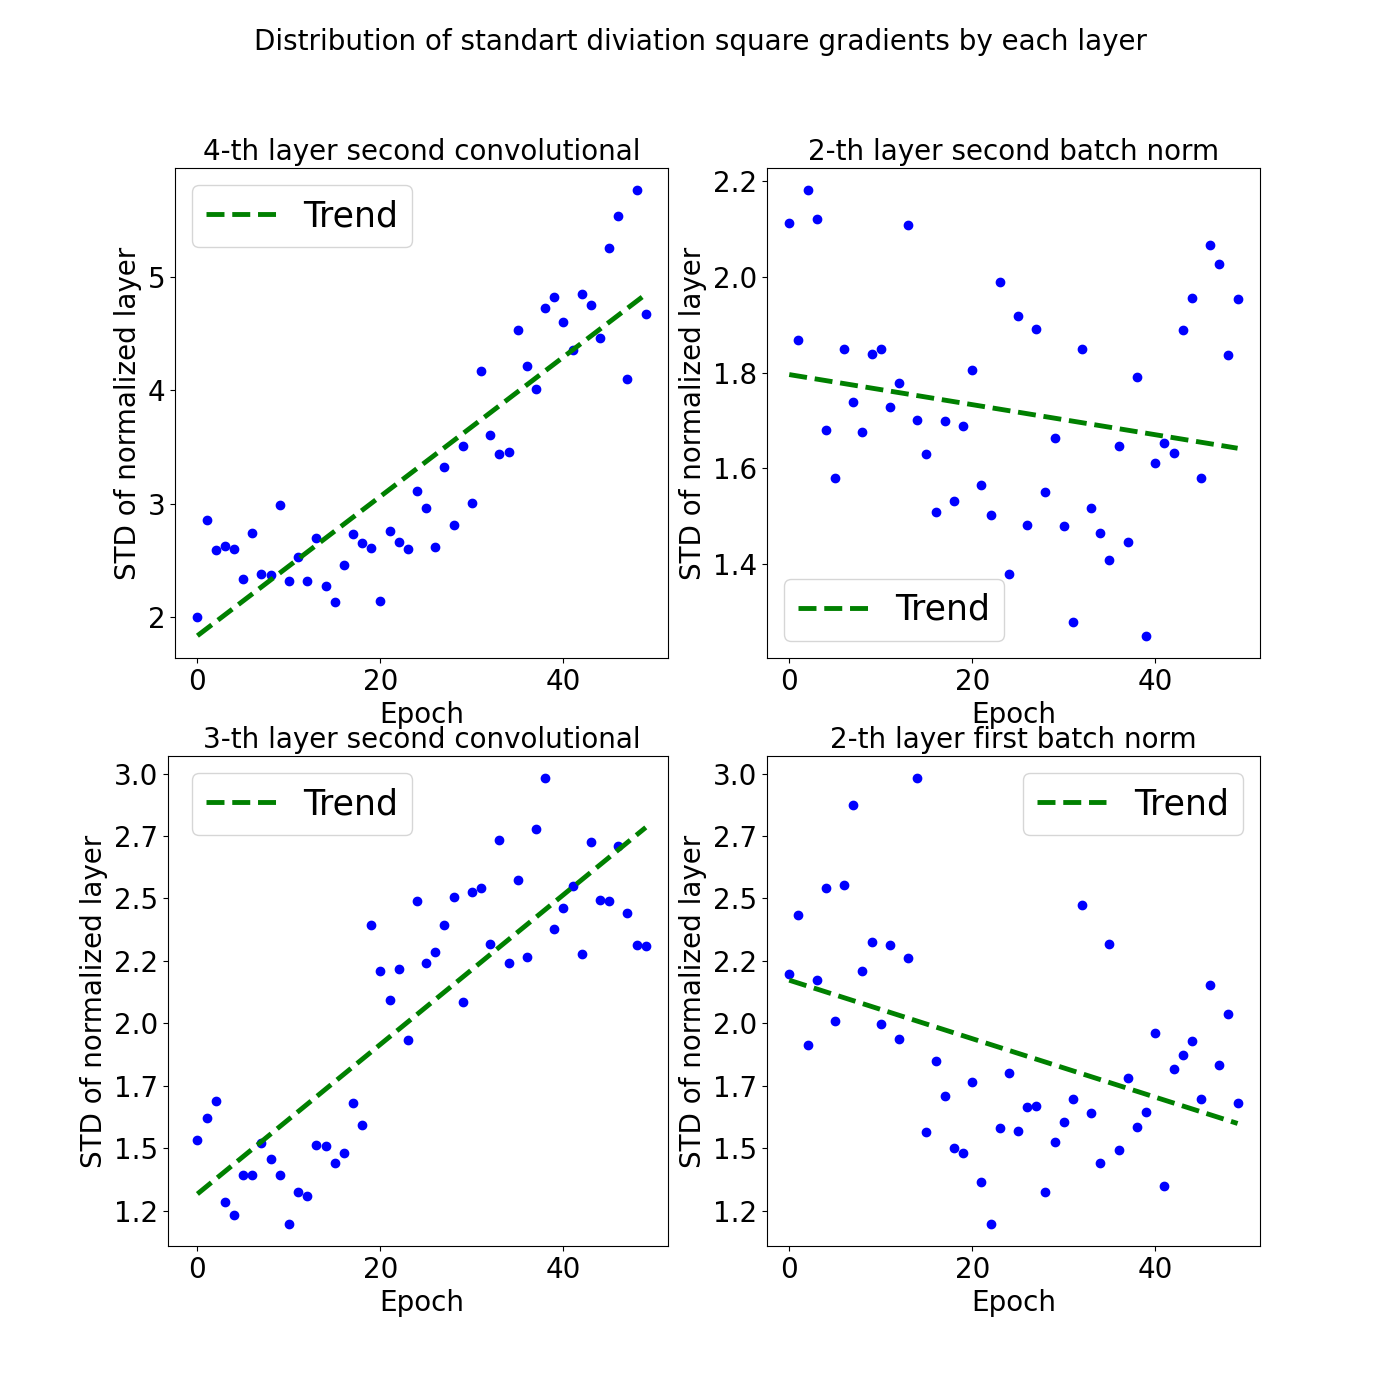
\includegraphics[width=\textwidth]{pictures/new_layers.png}
    \captionsetup{justification=centering,margin=2cm}
    \caption{Distribution of standard deviation of elements of matrix $D_t$ over epochs.}
    \label{fig:deviation}
\end{figure}

AdamW shows the worst results for the loss function, which repeats the results obtained with linear regression above. However, AdamW outperforms all other methods in terms of accuracy on the test dataset, demonstrating its generalization ability, as mentioned earlier.

We previously mentioned that the difference between the solutions of problems (4) and (9) can be bounded below by $||D_t - I||$.
This is why we were interested in investigating the deviation of the elements of $||D_t||$ during training.
Below, we examine the standard deviation of the normalized weights of the model across its layers, and we can observe certain trends in the convolutional and batch normalization layers that are framed in Figure \ref{fig:deviation}.

Deviation of the normalized weights in the convolutional layers has rising trend. Hence, difference
between solutions of different problems is bounded below and methods converge to a different optimums.

\section{Conclusion}

This study investigates the application of preconditioning methods with weight decay regularization.
We propose a novel approach that combines preconditioning methods with weight decaying and analyze the convergence of these methods under various conditions.
Theoretical and experimental analyses are conducted to investigate the solution to problem \eqref{F_tilde}, demonstrating that methods incorporating preconditioning and weight decaying do not converge to the optimum of the initial problem \eqref{F_big}.
We anticipate that this paper will be valuable for researchers in this field.
Further investigation is needed to understand the generalization ability of the introduced method and preconditioned methods with weight decaying.

\bibliographystyle{unsrtnat}
\bibliography{refs}

\section{Appendix}

\appendix
\label{sec:appendix}

\section{Experiments}

\begin{figure}[H]
\centering
    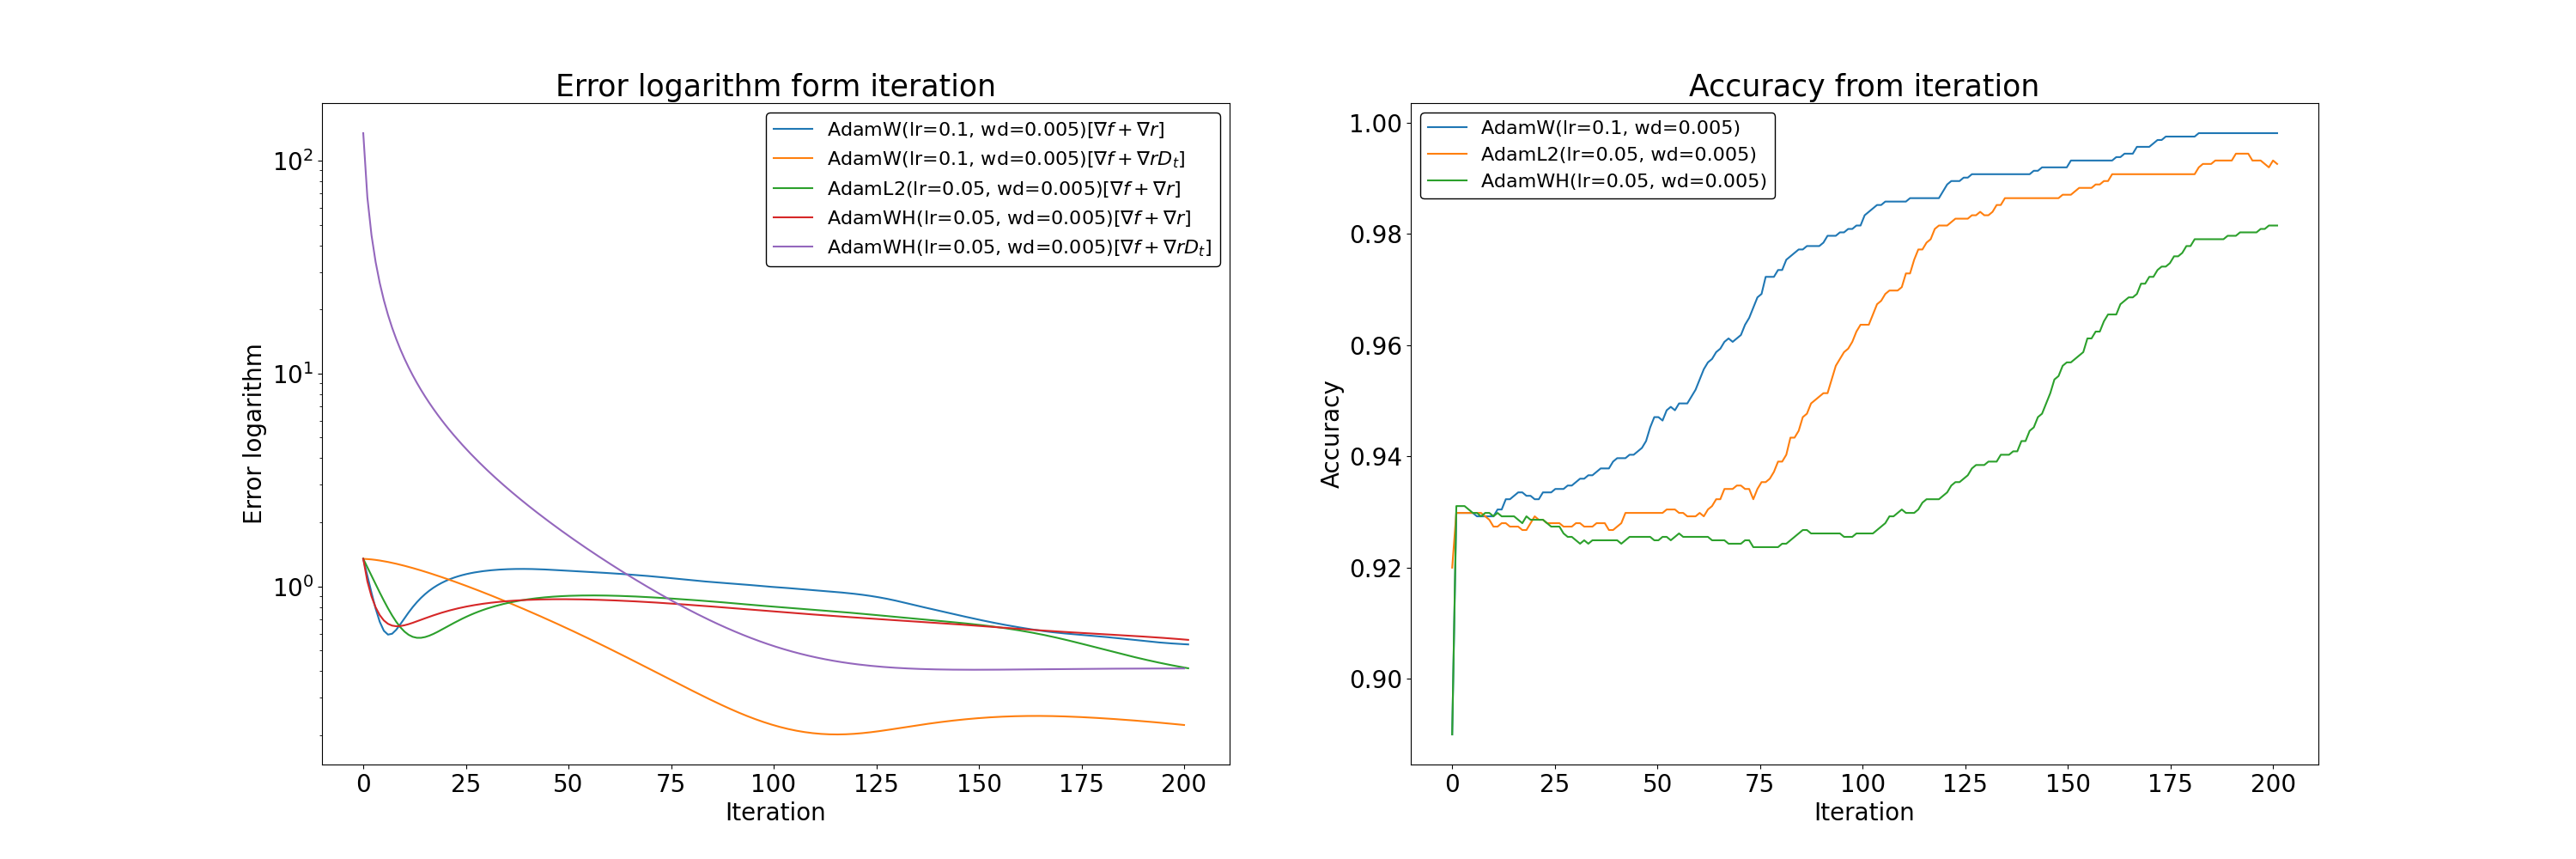
\includegraphics[width=0.93\textwidth]{pictures/mushrooms/main_adam.png}
    \caption{Different versions Adam algrorithms on dataset: mushrooms}
    \label{fig:main_mushrooms_adam}
\end{figure}

\begin{figure}[H]
\centering
    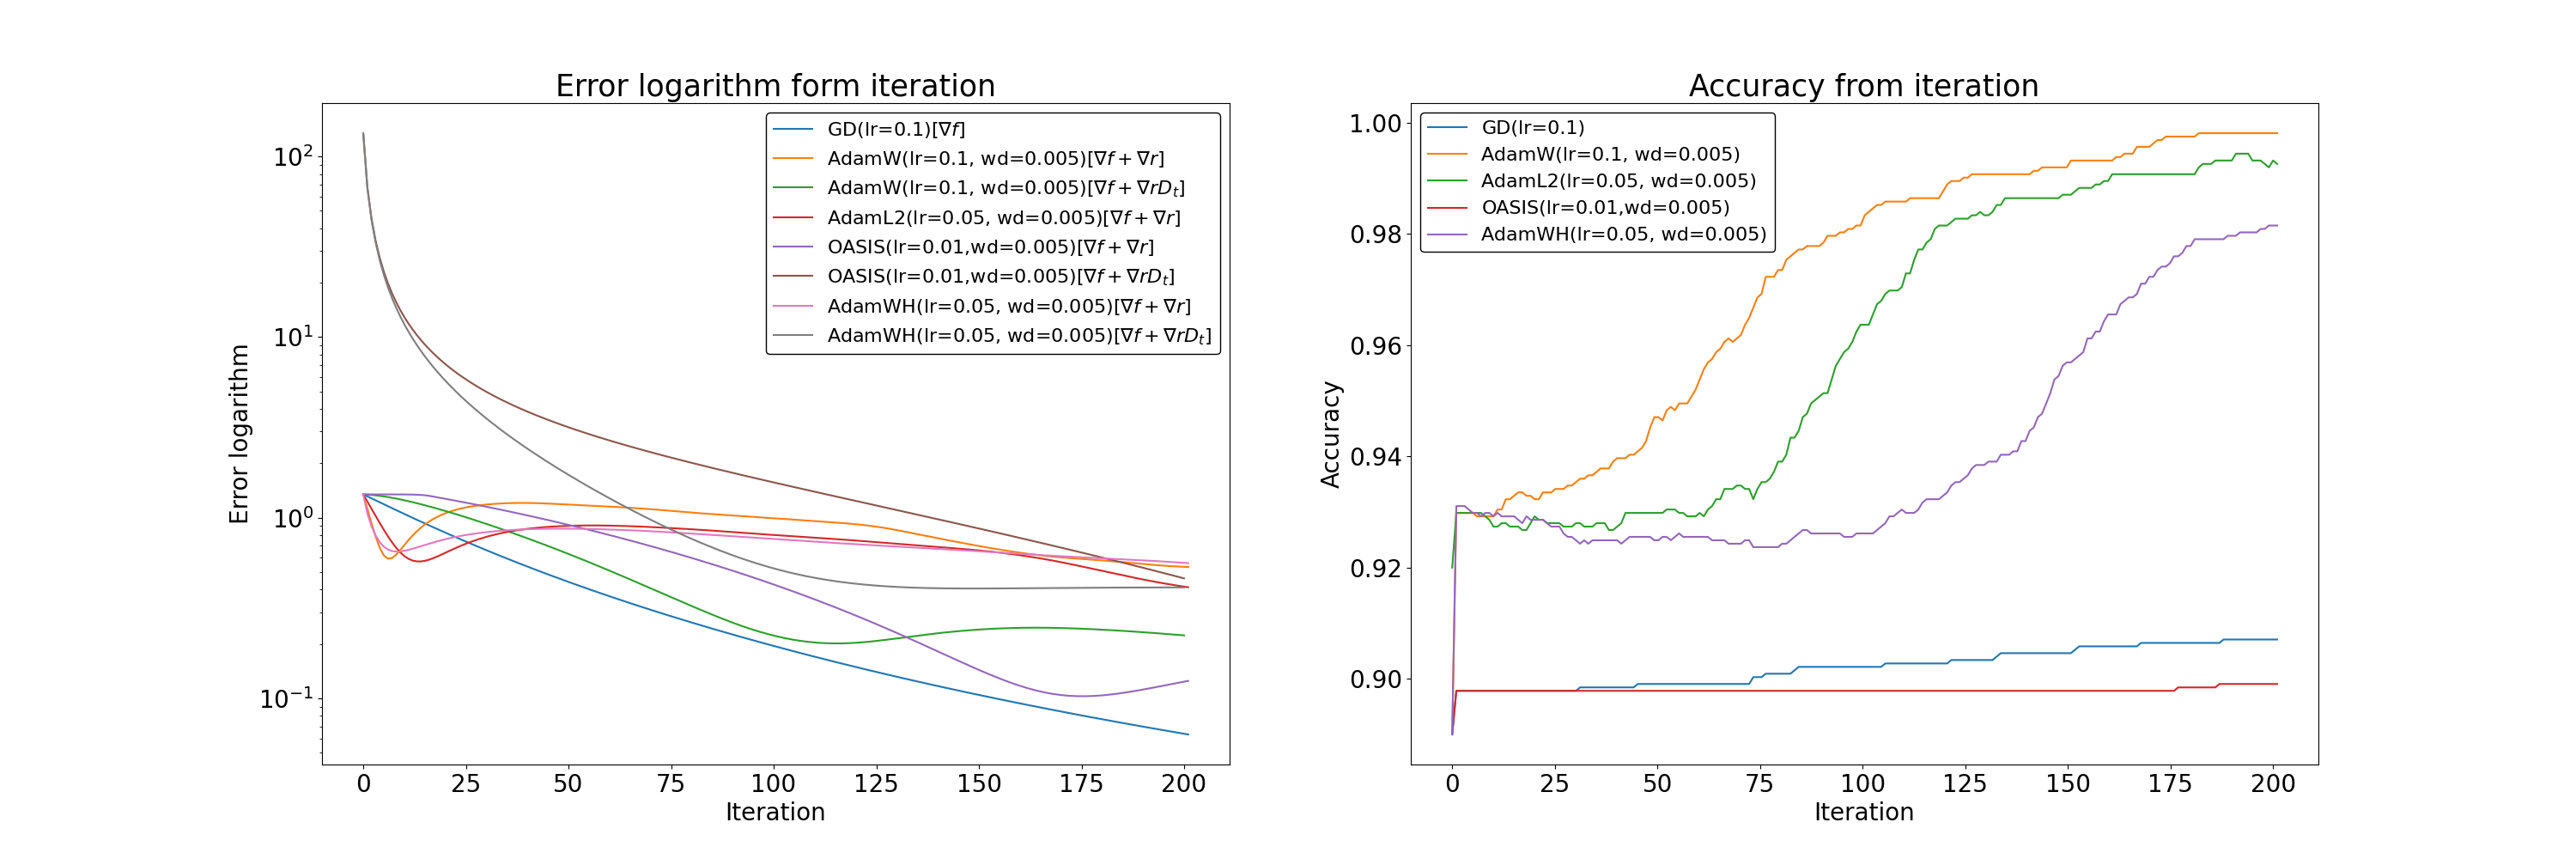
\includegraphics[width=0.93\textwidth]{pictures/mushrooms/main_mushrooms.png}
    \caption{Compare different optimization algorithms on dataset: mushrooms}
    \label{fig:main_mushrooms}
\end{figure}


\section{Proofs}

\subsection{Proofs of lemmas}


\begin{proof} (Proof of Lemma \ref{lemma:existence})

Using assumptions \ref{ass:regstruct}, \ref{ass:precondstruct} we can write the gradient of $\widetilde{r}$
    \begin{equation*}
        \nabla \widetilde{r} = \nabla \left( \sum_{i=1}^d D_t^i r_i(w_i) \right) = D_t \begin{pmatrix}
  r_1'(w_1) \\
  \vdots  \\
  r_d'(w_d)
 \end{pmatrix} = D_t \nabla r
    \end{equation*}
\end{proof}

\begin{proof} (Proof of Lemma \ref{lemma:tildesmoothness})

We can write definition of smoothness, using Lemma \ref{lemma:existence} and then apply \ref{ass:smoothness}
\begin{equation*}
    || \nabla \widetilde{r}(x) - \nabla \widetilde{r}(y) || =
    || \nabla \left( \sum_{i=1}^d D_t^i r_i(x_i) \right) - \nabla \left( \sum_{i=1}^d D_t^i r_i(y_i) \right) || =
    ||D_t \left( \nabla r(x) - \nabla r(y) \right)|| \le  ||D_t|| L_r
\end{equation*}
\end{proof}

\begin{proof} (Proof of lemma \ref{lemma:lowerbondF})

    Lets write definitions of solutions $w^*$, $\widetilde{w}^*$:
        \begin{equation*}
        \begin{cases}
            \nabla f (\widetilde{w}^*) + D_t \nabla r(\widetilde{w}^*) = 0\\
            \nabla f (w^*) + \nabla r(w^*) = 0\\
        \end{cases},
        \end{equation*}
        Then we are able to get lower bound from the definition of $L_F$-contentiousness of the function $F$.
        \begin{equation*}
        \|\widetilde{w}^* - w^* \| L_F \geq \| \nabla f (\widetilde{w}^*) + \nabla r(\widetilde{w}^*) - \nabla f (w^*) - \nabla r (w^*) \| \\
        = \| - D_t \nabla r (\widetilde{w}^*) + \nabla r(\widetilde{w}^*) \|  = \| \nabla r (\widetilde{w}^*) (I - D_t)\|
        \end{equation*}
\end{proof}



\subsection{Proofs of theorems}

\begin{proof} (Proof of \hyperref[theor:1]{theorem 1})
\label{proof:theorem1}

Let us use Assumption \eqref{ass:smoothness} for step $t$ and $t+1$:

\begin{equation} \label{eq1}
    f(w_{t+1}) \leq f(w_t) + \langle \nabla f(w_t), w_{t+1} - w_t \rangle + \frac{L_f}{2}||w_{t+1} - w_t ||^2,
\end{equation}
By definition for our algorithm we have:

\begin{equation*}
w_{t+1} - w_t = -\eta D_t^{-1} \nabla f(w_t) - \eta \nabla r(w_t).
\end{equation*}

From the previous expression , we select the gradient of the function

\begin{equation*}
\nabla f(w_t) = \frac{1}{\eta} D^t(w_t - w_{t+1}) - D^t \nabla r(w_t),
\end{equation*}

replace $\nabla f(w_t)$ in \ref{eq1} and by definition of matrix $D_t$, $I \preccurlyeq \frac{D_t}{\alpha}$
\begin{equation*}
    f(w_{t+1}) \leq f(w_t) + \langle \frac{1}{\eta}D_t(w_t - w_{t+1}) - D_t\nabla r(w_t), w_{t+1} - w_t \rangle + \frac{L_f}{2 \alpha} ||w_{t+1} - w_t||_{D_t}^2 = 
\end{equation*}

\begin{equation*}
    = f(w_t) + \left(\frac{L_f}{2 \alpha} - \frac{1}{\eta} \right) ||w_{t+1} - w_t||_{D_t}^2 - \langle D_t \nabla r(w_t), w_{t+1} - w_t \rangle,
\end{equation*}

using the notation of $\tilde{r} : \nabla \tilde{r} = D_t \nabla r(w_t)$,
we can rewrite step using the variable and Assumption \eqref{ass:smoothness}
\begin{equation*}
    \tilde{r}(w_{t+1}) \leq \tilde{r}(w_t) + \langle \nabla \tilde{r}(w_t), w_{t+1} - w_t \rangle + \frac{L_{\tilde{r}}}{2} ||w_{t+1} - w_t||_2^2
\end{equation*}

Let us replace the old regularization function with a new one

\begin{equation*}
    f(w_{t+1}) \leq f(w_t) + \left( \frac{L_f}{2\alpha} - \frac{1}{\eta} \right) ||w_{t+1} - w_t||_{D_t}^2 + \tilde{r}(w_t) - \tilde{r}(w_{t+1}) + \frac{\Gamma L_{\tilde{r}}}{2}||w_{t+1}-w_t||_{D_t}^2.
\end{equation*}

Now let us define a new loss function
$\tilde{F}(w) = f(w) + \tilde{r}(w)$, $F(w) = f(w) + r(w)$, ($\tilde{L}=L_f + \Gamma L_{\tilde{r} \alpha}$), we get:

\begin{equation*}
    \tilde{F}(w_{t+1}) \leq \tilde{F}(w_t) + \left( \frac{\tilde{L}}{2\alpha} - \frac{1}{\eta}  \right) ||w_{t+1} - w_t||_{D_t}^2,
\end{equation*}

we select the step in such a way that $ \frac{\tilde{L}}{2\alpha} - \frac{1}{\eta} < 0$,  $\eta < \frac{2 \alpha}{\tilde{L}}$
\begin{equation*}
    \left(\frac{1}{\eta} - \frac{\tilde{L}}{2\alpha}   \right) ||w_{t+1} - w_t||_{D_t}^2 \leq \tilde{F}(w_t) - \tilde{F}(w_{t+1}).
\end{equation*}

Let us sum up our inequalities and evaluate the left part from below
\begin{equation*}
    \frac{\eta^2  (T+1)}{\Gamma}\left(\frac{1}{\eta} - \frac{\tilde{L}}{2\alpha}   \right)\cdot\min_{k = 0, T} ||\nabla f(w_t) + \nabla \tilde{r}(w_t)||^2 \leq \frac{\eta^2}{\Gamma}\left(\frac{1}{\eta} - \frac{\tilde{L}}{2\alpha}   \right)\cdot\sum\limits_{t = 0}^T ||\nabla f(w_t) + \nabla \tilde{r}(w_t)||^2 \leq \tilde{F}(w_0) - \tilde{F}(w_*).
\end{equation*}

Moving everything to the right we get the following estimate

\begin{equation*}
    \min_{t = 0, T} ||\nabla f(w_t) + \nabla \tilde{r}(w_t)||^2 \leq \frac{(\tilde{F}(w_0) - \tilde{F}(w_*))\Gamma}{(\frac{1}{\eta} - \frac{\tilde{L}}{2\alpha}) \eta^2 (T+1)} = \varepsilon
\end{equation*}

\begin{equation*}
    T + 1 \geq \frac{\Delta_0 \Gamma}{(\frac{1}{\eta} - \frac{\tilde{L}}{2\alpha}) \eta^2 \varepsilon}.
\end{equation*}

We get an estimate for the number of steps required for a given accuracy
\begin{equation*}
      T = \mathcal{O}\left( \frac{2\Delta_0 \Gamma \alpha } {(2\alpha - \tilde{L}\eta) \eta \varepsilon} \right).
\end{equation*}
\end{proof}





\begin{proof} (Proof of \hyperref[theor:2]{theorem 2})
\label{proof:theorem2}

    
    The proof of this theorem will be similar to the previous one, the main difference is that we impose another Assumption \hyperref[ass:plcondition]{3} on the original function 
    Assume 
    \begin{equation*}
    \nabla \tilde{F} = \nabla f + \nabla \tilde{r}    
    \end{equation*}
    
    \begin{equation*}
    L_{f} + ||D_t||L_{r} = L_{\tilde{F}}        
    \end{equation*}
    rewrite step in terms of new function
    \begin{equation*}
    w_{t+1} - w_t = -\eta D_t^{-1} \nabla r(w_t) - \eta \nabla r(w_t) = -\eta D_t^{-1} (\nabla f + \nabla \tilde{r})(w_t) = -\eta D_t^{-1} \nabla \tilde{F}(w_t),
    \end{equation*}
    Then we write $\tilde{L}$-smoothness for $\tilde{F}$ 
    \begin{equation*}
        \tilde{F}(w_{t+1}) - \tilde{F}(w_t) \leq  \langle \nabla \tilde{F}(w_t), w_{t+1} - w_t \rangle + \frac{L_{\tilde{F}}}{2} ||w_{t+1} - w_t||^2,
    \end{equation*}
    then combine it together and use constraints on the matrix $\alpha \cdot I \preccurlyeq D_t \preccurlyeq \Gamma \cdot I$
    \begin{eqnarray*}
&& \        \tilde{F}(w_{t+1}) - \tilde{F}(w_t) \leq - \langle \frac{1}{\eta} D_t(w_{t+1} - w_t), w_{t+1} - w_t \rangle + \frac{L_{\tilde{F}}}{2} ||w_{t+1} - w_t||^2 = \left( \frac{L_{\tilde{F}}}{2 \alpha} - \frac{1}{\eta} \right) ||w_{t+1} - w_t||^2_{D_t} =
\notag\\& =&
\left(\frac{L_{\tilde{F}}}{2 \alpha} - \frac{1}{\eta} \right) ||w_{t+1} - w_t||^2_{D_t} = \left(\frac{L_{\tilde{F}}}{2 \alpha} - \frac{1}{\eta} \right) ||-\eta D_t^{-1} \nabla \tilde{F}(w_t)||_{D_t}^2  \leq \left(\frac{L_{\tilde{F}}}{2 \alpha} - \frac{1}{\eta} \right) \eta^2 ||\nabla \tilde{F}(w_t)||^2_{D_t^{-1}},
\end{eqnarray*}

    We use PL-condition \ref{ass:plcondition} for the function $\tilde{F}$:
    \begin{equation*}
        ||\nabla \tilde{F}(w_t)||_{D_t^{-1}}^2 \geq 2 \mu (\tilde{F}(w_t) - \tilde{F}^*),
    \end{equation*}
    
    subtract the exact solution from both parts and apply PL-condition
    \begin{equation*}
    \tilde{F}(w_{t}) -  F^* \ge \tilde{F}(w_{t+1}) - \tilde{F}^* + \left(\frac{1}{\eta} - \frac{L_{\tilde{F}}}{2 \alpha} \right) \eta^2 2 \mu (\tilde{F}(w_t) - \tilde{F}^*) = \left( 1 +  2 \mu \eta^2 \left(\frac{1}{\eta} - \frac{L_{\tilde{F}}}{2 \alpha} \right) \right) (\tilde{F}(w_{t+1}) - \tilde{F}^*).
    \end{equation*}

    Let us apply the expression for each step and use expression $\Delta_0 = \tilde{F}(w_0) - \tilde{F}(w_{*})$
    \begin{equation*}
    \varepsilon \ge \Delta_0 \left( 1 +  2 \mu \eta^2 \left(\frac{1}{\eta} - \frac{L_{\tilde{F}}}{2 \alpha} \right) \right)^{-T} \ge (\tilde{F}(w_{T}) - \tilde{F}^*),   
    \end{equation*}
    
    from this expression we get the necessary number of steps to get together with the error $\varepsilon$
    \begin{equation*}
    T = \frac{\ln \frac{\Delta_0}{\varepsilon}}{\ln{\left(1 + 2 \mu \eta^2 \left(\frac{1}{\eta} - \frac{L_{\tilde{F}}}{2 \alpha} \right) \right)}} \approx \frac{\ln \frac{\Delta_0}{\varepsilon}}{2 \mu \eta^2 \left( \frac{1}{\eta} - \frac{L_{\tilde{F}}}{2 \alpha}\right)}.
    \end{equation*}
    We get an estimate on the number of steps of the algorithm for a given error on the difference of the loss function
    \begin{equation*}
    T =  \mathcal{O}\left( \frac{\ln \frac{\Delta_0}{\varepsilon}}{2 \mu \eta^2(\frac{1}{\eta} - \frac{L_{\tilde{F}}}{2 \alpha})} \right)
    \end{equation*}
\end{proof}


\begin{proof} (Proof of \hyperref[theor:3]{theorem 3})
\label{proof:theorem3}

We start from $L$-smoothness of $f$ (Assumption \eqref{ass:smoothness}).
\begin{equation*}
    f(w_{t+1}) \leq f(w_t) + \langle \nabla f(w_t), w_{t+1} - w_t \rangle + \frac{L_f}{2}||w_{t+1}-w_t||_2^2
\end{equation*}

Next we substitute an update of $w$:
\begin{equation*}
    f(w_{t+1}) \leq f(w_t) + \langle \nabla f(w_t), w_{t+1} - w_t \rangle + \frac{L_f \eta^2}{2}||D_t^{-1}g_t + \nabla r(w_t)||_2^2 = 
\end{equation*}

Then we added and subtracted $D_t^{-1} \nabla f(w_t)$ under of the norm:
\begin{equation*}
    =  f(w_t) + \langle \nabla f(w_t), w_{t+1} - w_t \rangle + \frac{L_f \eta^2}{2}||D_t^{-1}g_t - D_t^{-1} \nabla f(w_t) + D_t^{-1} \nabla f(w_t) + \nabla r(w_t)||_2^2 = 
\end{equation*}

\begin{equation*}
    =  f(w_t) + \langle \nabla f(w_t), w_{t+1} - w_t \rangle + \frac{L_f \eta^2}{2}||D_t^{-1}g_t - D_t^{-1} \nabla f(w_t)||_2^2 + \frac{L_f \eta^2}{2}\langle D_t^{-1}g_t - D_t^{-1} \nabla f(w_t), D_t^{-1} \nabla f(w_t) + \nabla r(w_t) \rangle + 
\end{equation*}
\begin{equation*}
    + \frac{L_f \eta^2}{2} ||D_t^{-1} \nabla f(w_t) + \nabla r(w_t)||_2^2.
\end{equation*}

Then we take full expectation:
\begin{equation*}
    \mathbb{E} f(w_{t+1}) \leq \mathbb{E} f(w_t) + \frac{L_f \eta^2}{2} \mathbb{E} ||D_t^{-1}g_t - D_t^{-1}\nabla f(w_t)||_2^2 + \frac{L_f \eta^2}{2} \mathbb{E} \langle D_t^{-1}g_t - D_t^{-1} \nabla f(w_t), D_t^{-1} \nabla f(w_t) + \nabla r(w_t) \rangle
\end{equation*}
\begin{equation*}
    + \frac{L_f \eta^2}{2}\mathbb{E} ||D_t^{-1} \nabla f(w_t) + \nabla r(w_t)||_2^2.    
\end{equation*}

Using Assumption \hyperref[ass:expectations]{4}, $\mathbb{E} \left[D_t^{-1}(g_t - \nabla f(w_t)\right] = 0$, $||g_t - \nabla f (w_t)||_2^2 \leq \sigma^2$
\begin{equation*}
 \mathbb{E} f(w_{t+1}) \leq \mathbb{E} f(w_t) + \mathbb{E} \langle \nabla f(w_t), w_{t+1} - w_t \rangle + \frac{L_f \eta^2}{2 \alpha^2} \mathbb{E} ||g_t - \nabla f(w_t)||_2^2 + \frac{L_f \eta^2}{2\alpha^2} \mathbb{E}||\nabla f(w_t) + D_t \nabla r(w_t)||_2^2,
\end{equation*}
then apply second part of Assumption \hyperref[ass:expectations]{4}:
\begin{equation*}
 \mathbb{E} f(w_{t+1}) \leq \mathbb{E} f(w_t) + \mathbb{E} \langle \nabla f(w_t), w_{t+1} - w_t \rangle + \frac{L_f \eta^2\sigma^2}{2 \alpha^2}  + \frac{L_f \eta^2}{2\alpha^2} \mathbb{E}||\nabla f(w_t) + D_t \nabla r(w_t)||_2^2.
\end{equation*}

Then again use \hyperref[ass:expectations]{4}
$$
\nabla f(w_t) =\mathbb{E} g_t = \mathbb{E} \frac{1}{\eta}D_t(w_t - w_{t+1}) + D_t\nabla r(w_t)
$$
and put it in the inequality:
\begin{equation*}
    \mathbb{E} f(w_{t+1}) \leq \mathbb{E} f(w_t) + \mathbb{E} \langle \mathbb{E} \frac{1}{\eta}D_t(w_t - w_{t+1}) + D_t\nabla r(w_t), w_{t+1} - w_t \rangle + \frac{L_f \eta^2}{2 \alpha^2} \mathbb{E} ||\nabla f(w_t) + D_t \nabla r(w_t)||_2^2 + \frac{L_f \eta^2\sigma^2}{2 \alpha^2}.
\end{equation*}
Let's rewrite it in a convenient way:
\begin{equation*}
    \mathbb{E} f(w_{t+1}) \leq \mathbb{E} f(w_t) 
    -\frac{1}{\eta}\mathbb{E} ||w_{t+1} - w_t||_{D_t}^2 + \mathbb{E} \langle D_t \nabla r(w_t), w_{t+1} - w_t \rangle + \frac{L_f \eta^2}{2 \alpha^2} \mathbb{E} ||\nabla f(w_t) + D_t \nabla r(w_t)||_2^2 + \frac{L_f \eta^2\sigma^2}{2 \alpha^2} .
\end{equation*}

Using Lemma \hyperref[lemma:tildesmoothness]{2} about $L_{\tilde{r}}-smoothness$ of $\tilde r(w_t) = D_t \nabla r(w_t)$
\begin{equation*}
    \mathbb{E} f(w_{t+1}) \leq \mathbb{E} f(w_t) -\frac{1}{\eta} \mathbb{E} ||w_{t+1} - w_t||_{D_t}^2 + \mathbb{E} \tilde{r}(w_t) - \mathbb{E} \tilde{r}(w_{t+1}) + \frac{L_{\tilde{r}}}{2} \mathbb{E}||w_{t+1} - w_t||_2^2 + \frac{L_f \eta^2}{2 \alpha^2} \mathbb{E} ||\nabla f(w_t) + D_t \nabla r(w_t)||_2^2 +
\end{equation*}
\begin{equation*}
    + \frac{L_f \eta^2\sigma^2}{2 \alpha^2}.
\end{equation*}
Then we apply $L_{\tilde{F}}-smoothness$ and get:
\begin{equation*}
    \mathbb{E} \left( f(w_t) + \tilde{r}(w_t) \right) \leq \mathbb{E} \left( f(w_{t+1}) + \tilde{r} (w_{t+1})\right) + \mathbb{E}||w_{t+1} - w_t||_{D_t}^2 \left(-\frac{1}{\eta} + \frac{ \Gamma L_{\tilde{r}}}{2} + \frac{\Gamma L_{\tilde{F} }L_{f}\eta^2 }{2\alpha^2} \right) + \frac{L_f \eta^2 \sigma^2}{2 \alpha^2}.
\end{equation*}

And with restrictions on $\eta$ such that: $\left(-\frac{1}{\eta} + \frac{ \Gamma L_{\tilde{r}}}{2} + \frac{\Gamma L_{\tilde{F} }L_{f}\eta^2 }{2\alpha^2} \right) \leq 0$:
\begin{equation*}
   \left(-\frac{1}{\eta} + \frac{ \Gamma L_{\tilde{r}}}{2} + \frac{\Gamma L_{\tilde{F} }L_{f}\eta^2 }{2\alpha^2} \right) \mathbb{E} ||w_{t+1} - w_{t}||_{D_t}^2 \leq \mathbb{E} \tilde{F}(w_t) - \mathbb{E}  \tilde{F} (w_{t+1}) + \frac{L_f \eta^2 \sigma^2}{2\alpha^2}.
\end{equation*}

Then using the expectation and $L_{\tilde{F}}-smoothness$:
\begin{equation*}
    \frac{T}{\Gamma} \left(\frac{1}{\eta} - \frac{ \Gamma L_{\tilde{r}}}{2} - \frac{\Gamma L_{\tilde{F} }L_{f}\eta^2}{2\alpha^2} \right) \min_{k = \overline{0, T-1}} ||\nabla f(w_t) +\nabla \tilde{r} (w_t)||_2^2 \leq \frac{1}{\Gamma} \cdot \left(\frac{1}{\eta} - \frac{ \Gamma L_{\tilde{r}}}{2} - \frac{\Gamma L_{\tilde{F} }L_{f}\eta^2}{2\alpha^2} \right) \sum\limits_{i=0}^{T-1} ||\nabla f(w_t) + \nabla \tilde{r}(w_t)||_2^2 
\end{equation*}
\begin{equation*}
    \leq \tilde{F}(w_0) - \tilde{F}(w_*) + T\cdot\frac{L_f \eta^2\sigma^2}{2\alpha^2} \leq \varepsilon
\end{equation*}
Choose $\eta \sim \frac{(\tilde{F}(w_0) - \tilde{F}(w_*))\alpha^2}{L_f\sigma^2}$, we get an estimate the number of steps of the algorithm for a given error $\varepsilon$:
\begin{equation*}
        T =  \mathcal{O}\left( \frac{\Gamma \Delta_0}{\left(\frac{1}{\eta} - \frac{ \Gamma L_{\tilde{r}}}{2} - \frac{\Gamma L_{\tilde{F} }L_{f}\eta^2}{2\alpha^2} \right) \varepsilon} \right)
\end{equation*}

\end{proof}

\end{document}
